% !TeX root = it-governance-risk-compliance.tex
% !TeX encoding = UTF-8
\chapter{Risiko Pihak Ketiga dan Cloud}

\section*{Tujuan Pembelajaran}
\begin{itemize}
  \item Menyusun siklus hidup manajemen risiko pihak ketiga, mulai dari uji tuntas sampai
  pemutusan kontrak.
  \item Memetakan pembagian tanggung jawab keamanan antara organisasi dan penyedia cloud.
  \item Menyusun penilaian dampak pelindungan data pribadi untuk alur berbagi data dengan mitra.
\end{itemize}

\section{Pendahuluan}

Kebocoran dapat terjadi di vendor, tetapi pasien tetap meminta pertanggungjawaban organisasi
yang melayaninya. Insiden Medikara pada 2025 memperlihatkan pola itu. Pada data latihan Bab 7,
kontrak pekerjaan vendor sudah selesai, tetapi akun dukungan tetap aktif. Selama 8 malam, akun
itu melakukan 155 panggilan per malam dan membaca 1.240 rekam kunjungan pada dua rumah sakit.
Medikara baru mengetahuinya pada hari ke-11 lewat keluhan pasien. Risiko pihak ketiga karena itu
tidak selesai ketika kontrak ditandatangani atau sertifikat penyedia diterima.

Strategi Medikara membuka kerja sama dengan klinik, asuransi, laboratorium, apotek daring, dan
penyedia cloud. Setiap hubungan mempunyai data, ketergantungan, serta hak keputusan berbeda.
Pemilihan mitra harus diikuti kendali selama hubungan berlangsung dan cara keluar yang dapat
diuji. Bab 8 sudah menetapkan targetnya: Paket A menuntut 11 dari 11 butir perjanjian vendor,
dan Paket C menuntut laporan vendor dalam 12 jam. Bab ini menjelaskan cara mencapainya. Hasil
kerjanya adalah kerangka pihak ketiga, matriks tanggung jawab cloud, dan penilaian dampak
pelindungan data pribadi, atau \textit{Data Protection Impact Assessment} (DPIA), untuk tonggak
C3 capstone.

Bab ini memakai ISO/IEC 27036-2:2022 dari International Organization for Standardization (ISO)
dan International Electrotechnical Commission (IEC) untuk hubungan pemasok. Panduan National
Institute of Standards and Technology (NIST) SP 800-161 Rev. 1 dipakai untuk risiko rantai
pasok, NIST SP 800-145 untuk definisi cloud, serta Cloud Controls Matrix (CCM) dan Consensus
Assessments Initiative Questionnaire (CAIQ) dari Cloud Security Alliance (CSA) untuk penilaian
cloud. Penilaian dampak merujuk Undang-Undang Nomor 27 Tahun 2022 tentang Pelindungan Data
Pribadi (UU PDP). Naskah ISO berbayar, sehingga isinya ditulis secara umum. Pemetaan tanggung
jawab dan klausul contoh adalah rancangan pembelajaran yang harus disesuaikan dengan layanan
nyata, bukan nasihat hukum
\cite{c09-iso27036,c09-nist-sp800161,c09-nist-sp800145,c09-ccm,uu27-2022-pdp}.

\IfFileExists{../figures/ch09-diagram-konsep.png}{%

Gambar \ref{fig:ch09-ilustrasi-bab} merangkum hubungan komponen dan konsep utama bab ini.
\begin{figure}[!htb]
  \centering
  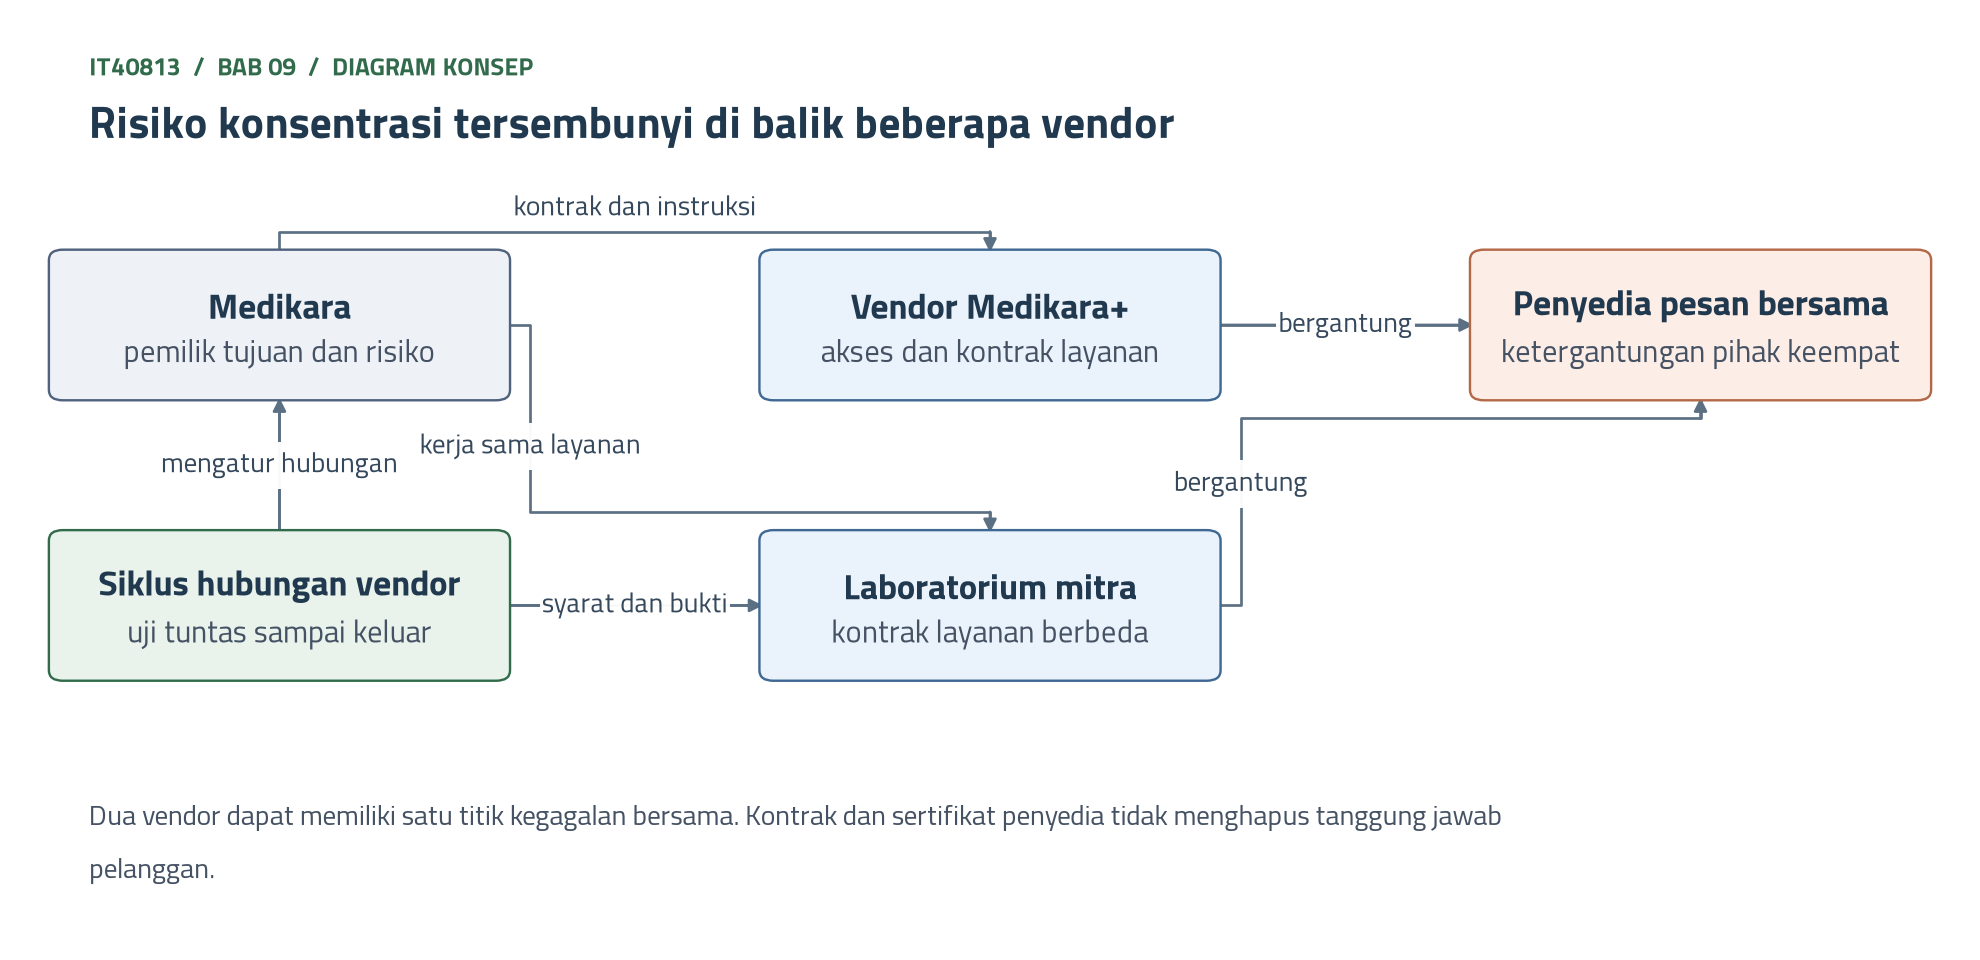
\includegraphics[width=\textwidth]{../figures/ch09-diagram-konsep.png}
  \caption{Risiko konsentrasi tersembunyi di balik beberapa vendor}
  \label{fig:ch09-ilustrasi-bab}
\end{figure}
}{}

\section{Rantai Pasok Digital dan Konsentrasi Risiko}

\subsection*{Pihak ketiga dan pihak keempat}

Pihak ketiga mencakup vendor aplikasi, penyedia cloud, mitra data, dan layanan pendukung. Pihak
keempat adalah pemasok yang dipakai pihak ketiga. NIST CSF 2.0 (Cybersecurity Framework) menyebut
teknologi bergantung pada ekosistem pasok yang saling terhubung, dengan beberapa lapis alih daya
\cite{nistcsf2}. Ketergantungan karena itu perlu ditelusuri melampaui nama vendor. Dua kontrak
berbeda dapat bergantung pada pusat data atau layanan identitas yang sama.

Analogi pemasok kantin menunjukkan konsentrasi. Dua pedagang yang membeli bahan dari gudang yang
sama tidak memberi keragaman pasokan ketika gudangnya tutup. Jumlah kontrak tidak sama dengan
jumlah sumber daya yang independen.

Dua contoh menuntut penelusuran lebih jauh:
\begin{enumerate}
  \item Misalkan vendor Medikara+ dan laboratorium mitra memakai penyedia pesan yang sama.
  Layanan pesan itu tersedia 99,5 persen dari 8.760 jam per tahun, sehingga gangguannya 43,8 jam
  per tahun. Bila kedua jalur benar-benar terpisah dan gangguannya tidak saling terkait, gangguan
  bersamaan hanya 0,5 persen dikali 0,5 persen, atau 0,0025 persen dari waktu. Angka itu setara
  sekitar 13 menit per tahun. Bila penyedianya sama, gangguan bersamaan menjadi 43,8 jam, atau
  200 kali lipat. Pengingat 336.000 janji temu per tahun ikut terganggu sekitar 0,5 persen, atau
  1.680 janji temu. Register Bab 5 mencatat skenario ini sebagai R-08 dengan skor
  $2 \times 4 = 8$.
  \item Misalkan cadangan ditempatkan di akun cloud yang sama dengan produksi. Akun yang diretas
  dapat membuat kedua salinan tidak dapat digunakan, meskipun medianya berbeda. Bab 3 mencatat
  144 uji pemulihan per tahun, yaitu 36 fasilitas dikali 4 uji. Seluruh uji itu dapat lulus tanpa
  menjawab skenario ini, bila setiap uji memakai akun pengelola yang sama. Bab 10 memakai temuan
  ini untuk R-05.
\end{enumerate}

Gambar~\ref{fig:ch09-peta} memperlihatkan peta ketergantungan pengandaian untuk lima hubungan
Medikara. Tabel~\ref{tab:ch09-rantai} merangkum pertanyaan yang perlu dijawab pada tiap hubungan.
Dari lima hubungan itu, penyedia pesan dan layanan identitas masing-masing dipakai dua hubungan.
V-01 menyentuh keduanya dan juga memakai V-02, sehingga vendor Medikara+ memiliki 3 penyedia
pendukung. Bab 7 memisalkan angka yang sama: Medikara perlu menunjukkan 3 persetujuan tertulis.

\begin{figure}[!htb]
  \centering
  \begin{tikzpicture}[
  font=\scriptsize,
  execute at begin node={\hyphenpenalty=10000},
  induk/.style={draw, rounded corners, align=center, text width=1.8cm,
    minimum height=1.3cm, fill=praditagreen!15},
  tahap/.style={draw, rounded corners, align=center, text width=3.1cm,
    minimum height=0.62cm, fill=blue!8},
  lanjut/.style={draw, rounded corners, align=center, text width=3.4cm,
    minimum height=0.62cm, fill=orange!12},
  masalah/.style={draw, rounded corners, align=center, text width=3.4cm,
    minimum height=0.9cm, fill=red!22},
  panah/.style={-{Stealth[length=2mm]}, thick}]
  \node[font=\scriptsize\bfseries] at (0,2.75) {Organisasi};
  \node[font=\scriptsize\bfseries] at (3.6,2.75) {Pihak ketiga};
  \node[font=\scriptsize\bfseries] at (8.1,2.75) {Pihak keempat};
  \node[induk] (m) at (0,0)
    {Medikara\\{\tiny\mdseries pemilik tujuan dan risiko}};
  \node[tahap] (v3) at (3.6,2) {V-03 Laboratorium mitra};
  \node[tahap] (v1) at (3.6,1) {V-01 Vendor Medikara+};
  \node[tahap] (v2) at (3.6,0) {V-02 Penyedia cloud};
  \node[tahap] (v4) at (3.6,-1) {V-04 Mitra asuransi};
  \node[tahap] (v5) at (3.6,-2) {V-05 Apotek daring};
  \node[masalah] (p1) at (8.1,1.6)
    {Penyedia pesan bersama\\{\tiny\mdseries titik kegagalan V-01 dan V-03}};
  \node[masalah] (p2) at (8.1,0.3)
    {Layanan identitas bersama\\{\tiny\mdseries titik kegagalan V-01 dan V-02}};
  \node[lanjut] (p3) at (8.1,-1) {Pengolah klaim};
  \node[lanjut] (p4) at (8.1,-2) {Kurir obat};
  \draw[panah] (m.east) -- (v3.west);
  \draw[panah] (m.east) -- (v1.west);
  \draw[panah] (m.east) -- (v2.west);
  \draw[panah] (m.east) -- (v4.west);
  \draw[panah] (m.east) -- (v5.west);
  \draw[panah] (v1.south) -- (v2.north);
  \draw[panah] (v3.east) -- (p1.west);
  \draw[panah] (v1.east) -- (p1.west);
  \draw[panah] (v1.east) -- (p2.west);
  \draw[panah] (v2.east) -- (p2.west);
  \draw[panah] (v4.east) -- (p3.west);
  \draw[panah] (v5.east) -- (p4.west);
\end{tikzpicture}

  \caption{Peta ketergantungan pihak ketiga dan pihak keempat (misalkan)}
  \label{fig:ch09-peta}
\end{figure}

\begin{table}[!htb]
  \centering\small
  \caption{Ketergantungan yang perlu ditelusuri (misalkan)}\label{tab:ch09-rantai}
  \begin{tabularx}{\textwidth}{|>{\raggedright\arraybackslash}X|>{\raggedright\arraybackslash}X|>{\raggedright\arraybackslash}X|}
    \hline
    \textbf{Hubungan} & \textbf{Pihak lanjutan} & \textbf{Pertanyaan} \\ \hline
    Vendor Medikara+ & Penyedia cloud, identitas, pesan, dan staf dukungan & Siapa dapat mengakses
    data, dan dari mana? \\ \hline
    Laboratorium mitra & Penyedia pesan bersama & Apakah ada titik kegagalan bersama? \\ \hline
    Cadangan data & Identitas dan akun pengelola & Apakah pemulihan tetap mungkin saat akun utama
    gagal? \\ \hline
    Mitra asuransi & Pengolah klaim & Siapa lagi menerima data klaim, dan untuk tujuan apa? \\
    \hline
    Apotek daring & Kurir obat & Data apa yang sampai ke kurir? \\ \hline
  \end{tabularx}
\end{table}

Dua hal sering tertukar: jumlah kontrak dan jumlah sumber daya yang independen. Pembagiannya
begini. Lima kontrak terlihat seperti lima pilihan. Bila dua di antaranya berhenti karena satu
penyedia yang sama, pilihannya tinggal tiga pada saat gangguan. Temuan ini punya dua konsekuensi.
Pertama, Medikara memerlukan inventaris layanan pemasok, yang pada NIST CSF tercantum sebagai
ID.AM-04 \cite{nistcsf2}. Kedua, kontrak harus mewajibkan vendor menyebut subprosesornya. Istilah
subprosesor pada bab ini sama dengan ``prosesor lain'' pada Pasal 51 ayat (5) UU PDP
\cite{uu27-2022-pdp}.

Diagram konsep pada awal bab meringkas pola itu. Medikara memegang tujuan dan risiko. Vendor
Medikara+ dan laboratorium mitra terikat kontrak layanan yang berbeda, tetapi keduanya bergantung
pada penyedia pesan bersama. Siklus hubungan vendor, dari uji tuntas sampai keluar, mengatur
hubungan itu lewat syarat dan bukti.

\subsection*{Membaca kejadian dan laporan industri}

Pertanyaan kemudian muncul: seberapa besar akibat pihak ketiga pada layanan kesehatan? Dua
kejadian dan satu laporan memberi pembacaan yang berbeda:
\begin{enumerate}
  \item Change Healthcare, Amerika Serikat. American Hospital Association (AHA) menyebut perusahaan
  ini memproses 15 miliar transaksi kesehatan per tahun, termasuk pemeriksaan kepesertaan,
  farmasi, klaim, dan pembayaran. Serangan terjadi pada 21 Februari 2024. Survei AHA pada 9 sampai
  12 Maret 2024 terhadap hampir 1.000 rumah sakit mencatat 94 persen mengalami dampak keuangan, 83
  persen dampak pada arus kas, dan 74 persen dampak pada pelayanan langsung pasien
  \cite{c09-aha-change}. Satu pihak ketiga yang berhenti dapat menyentuh banyak rumah sakit
  sekaligus.
  \item Synnovis, Inggris. NHS England London melaporkan serangan \textit{ransomware} pada 3 Juni
  2024 terhadap laboratorium patologi yang memproses tes darah bagi organisasi National Health
  Service (NHS), terutama di London bagian tenggara. Laporan mingguannya mencatat janji rawat jalan
  dan tindakan elektif yang ditunda pada dua \textit{trust} rumah sakit, dengan data manajemen yang
  belum diverifikasi \cite{c09-nhs-synnovis}. Angka rincinya tidak dikutip di sini, karena halaman
  laporan tidak dapat dibaca utuh saat pemeriksaan. Medikara memiliki laboratorium rujukan dan
  membuka kerja sama laboratorium mitra, sehingga polanya relevan.
\end{enumerate}

Laporan industri memberi gambaran lebih luas. Ringkasan WaterISAC atas Verizon Data Breach
Investigations Report (DBIR) 2026 menyebut keterlibatan pihak ketiga mencapai 48 persen
pelanggaran, naik 60 persen dari tahun sebelumnya \cite{c01-verizon-dbir2026,c09-waterisac-dbir}.
Data laporan industri dapat memberi konteks, tetapi persentase global tidak langsung menjadi
peluang insiden Medikara. Angka 48 persen adalah bagian dari seluruh pelanggaran yang dilaporkan,
bukan peluang satu rumah sakit mengalami insiden. Bab 5 tetap memakai peluang R-01 sebesar 0,2
per tahun, karena angka itu dinilai dari bukti Medikara.

Tabel~\ref{tab:ch09-pembacaan} merangkum cara membaca ketiga sumber. Tim memisahkan hasil survei,
definisi kejadian, dan bukti organisasi sebelum memakainya untuk keputusan risiko.

\begin{table}[!htb]
  \centering\small
  \caption{Membaca tiga sumber tentang risiko pihak ketiga}\label{tab:ch09-pembacaan}
  \begin{tabularx}{\textwidth}{|>{\raggedright\arraybackslash}p{0.2\textwidth}|>{\raggedright\arraybackslash}p{0.2\textwidth}|>{\raggedright\arraybackslash}X|>{\raggedright\arraybackslash}X|}
    \hline
    \textbf{Sumber} & \textbf{Jenis data} & \textbf{Yang berguna} & \textbf{Batas pembacaan} \\
    \hline
    Survei AHA & Laporan mandiri, beberapa pekan setelah serangan & Bentuk dampak pada kas dan
    pelayanan & Dibuat asosiasi rumah sakit; sistem pembiayaannya berbeda \\ \hline
    NHS England London & Data manajemen mingguan yang belum diverifikasi & Dampak dinyatakan dalam
    janji dan tindakan & Angka sementara; ukuran layanan berbeda \\ \hline
    DBIR 2026 lewat WaterISAC & Ringkasan laporan industri global & Tren keterlibatan pihak ketiga
    & Bagian dari pelanggaran, bukan peluang; definisi perlu dibaca pada laporan asli \\ \hline
  \end{tabularx}
\end{table}

\section{Siklus Hidup Risiko Pihak Ketiga}

\subsection*{Dari klasifikasi sampai keluar}

Manajemen pemasok dimulai sebelum pemilihan, dilanjutkan dengan kontrak, penerapan, pemantauan,
perubahan, dan penghentian. ISO/IEC 27036-2:2022 membahas persyaratan hubungan pengadaan dan
pemasok \cite{c09-iso27036}. NIST SP 800-161 Rev. 1 membahas identifikasi, penilaian, dan
pengurangan risiko rantai pasok siber pada semua tingkat organisasi \cite{c09-nist-sp800161}.
NIST CSF 2.0 merumuskan hasil yang dituju pada kategori GV.SC, dan menyebut SP 800-161 sebagai
bacaan mendalam \cite{nistcsf2}. Bab 8 menargetkan objektif COBIT APO10 \textit{Managed vendors}
pada tingkat 3 \cite{cobit2019-intro}.

Analogi menyewa kendaraan memperjelas siklusnya. Penyewa memeriksa kondisi sebelum menerima,
mencatat aturan penggunaan, memantau gangguan, lalu memeriksa keadaan saat mengembalikan. Tanda
tangan awal tidak menyelesaikan seluruh tanggung jawab.

Gambar~\ref{fig:ch09-siklus} memperlihatkan siklus kendali pihak ketiga dari klasifikasi sampai
keluar. Tabel~\ref{tab:ch09-siklus} memasangkan tiap tahap dengan hasil NIST CSF dan bukti pada
Medikara. Rumusan hasil pada tabel adalah ringkasan bab. Dari enam baris itu, hanya GV.SC-07 yang
masuk profil target Bab 8. Lima baris lain dipakai sebagai pertanyaan kerja, tanpa mengubah profil
16 dari 106 subkategori.

\begin{figure}[!htb]
  \centering
  \begin{tikzpicture}[
  font=\scriptsize,
  execute at begin node={\hyphenpenalty=10000},
  tahap/.style={draw, rounded corners, align=center, text width=1.85cm,
    minimum height=1.2cm, fill=blue!8},
  catatan/.style={align=center, font=\tiny\mdseries},
  panah/.style={-{Stealth[length=2mm]}, thick}]
  \node[tahap] (n0) at (0,0) {Klasifikasi\\{\tiny\mdseries GV.SC-04}};
  \node[tahap] (n1) at (2.5,0) {Uji tuntas\\{\tiny\mdseries GV.SC-06}};
  \node[tahap, fill=orange!12] (n2) at (5,0) {Kontrak\\{\tiny\mdseries GV.SC-05}};
  \node[tahap] (n3) at (7.5,0) {Penerapan dan pemantauan\\{\tiny\mdseries GV.SC-07}};
  \node[tahap, fill=green!10] (n4) at (10,0) {Keluar dan verifikasi\\{\tiny\mdseries GV.SC-10}};
  \node[tahap, fill=red!22] (ins) at (7.5,-2) {Insiden bersama\\{\tiny\mdseries GV.SC-08}};
  \draw[panah] (n0) -- (n1);
  \draw[panah] (n1) -- (n2);
  \draw[panah] (n2) -- (n3);
  \draw[panah] (n3) -- (n4);
  \draw[panah] (n3) -- (ins);
  \draw[panah, rounded corners] (ins.west) -| (n2.south);
  \draw[panah, rounded corners] (n3.north) -- ++(0,0.45) -| (n0.north);
  \node[catatan] at (3.75,1.32)
    {perubahan tujuan, subprosesor, lokasi, atau skala memicu klasifikasi ulang};
  \node[catatan, anchor=east] at (6.3,-2.2) {temuan memperbaiki klausul};
\end{tikzpicture}

  \caption{Siklus kendali pihak ketiga dari klasifikasi sampai keluar}
  \label{fig:ch09-siklus}
\end{figure}

\begin{table}[!htb]
  \centering\small
  \caption{Tahap siklus, hasil NIST CSF, dan bukti Medikara (misalkan)}\label{tab:ch09-siklus}
  \begin{tabularx}{\textwidth}{|>{\raggedright\arraybackslash}p{0.19\textwidth}|>{\raggedright\arraybackslash}p{0.14\textwidth}|>{\raggedright\arraybackslash}X|>{\raggedright\arraybackslash}X|}
    \hline
    \textbf{Tahap} & \textbf{Hasil} & \textbf{Ringkasan hasil} & \textbf{Bukti pada Medikara} \\
    \hline
    Klasifikasi & GV.SC-04 & Pemasok dikenal dan diprioritaskan menurut kekritisan & Register
    pemasok dengan skor \\ \hline
    Uji tuntas & GV.SC-06 & Perencanaan dan uji tuntas sebelum hubungan resmi & Kuesioner beserta
    bukti dan cakupan \\ \hline
    Kontrak & GV.SC-05 & Persyaratan masuk kontrak dan perjanjian & 11 dari 11 butir; klausul K-05
    \\ \hline
    Penerapan dan pemantauan & GV.SC-07 & Risiko dinilai dan dipantau sepanjang hubungan & 60 dari
    60 catatan AC-01; tinjauan triwulanan \\ \hline
    Insiden bersama & GV.SC-08 & Pemasok dilibatkan dalam rencana insiden dan pemulihan & 2 latihan
    per tahun; laporan 12 jam \\ \hline
    Keluar & GV.SC-10 & Rencana mencakup kegiatan setelah hubungan berakhir & Hasil uji ekspor dan
    bukti penghapusan \\ \hline
  \end{tabularx}
\end{table}

\subsection*{Klasifikasi: seberapa dalam pemeriksaannya?}

Klasifikasi menentukan kedalaman pemeriksaan. Tiga pertanyaan cukup untuk memulai: data apa yang
disentuh, layanan apa yang berhenti bila pihak itu gagal, dan seberapa sulit menggantinya.
Pemeriksaan yang sama untuk semua pemasok memboroskan tenaga pada pemasok kecil dan mengurangi
perhatian pada pemasok kritis.

Analogi tamu rumah sakit membantu. Pengantar bunga cukup mendaftar di lobi. Teknisi yang masuk
ruang obat perlu surat tugas, pendamping, dan catatan keluar. Keduanya tamu, tetapi risikonya
berbeda.

Dua contoh menentukan tingkat pemeriksaan:
\begin{enumerate}
  \item Misalkan penyedia cetak materi umum tidak menerima data pribadi dan mudah diganti. Skornya
  1 dari 9, sehingga pemeriksaan dasar memadai. Vendor Medikara+ mengolah data kesehatan untuk
  28.000 janji temu per bulan dan mendukung layanan lintas fasilitas. Skornya 9 dari 9. Uji akses,
  insiden, pemulihan, subprosesor, serta strategi keluar menjadi prioritas.
  \item Misalkan register pemasok memuat 40 hubungan: 5 tingkat terperinci, 12 menengah, dan 23
  dasar. Pemeriksaan memakan 40, 16, dan 4 jam per hubungan. Totalnya 200 tambah 192 tambah 92,
  atau 484 jam, yaitu Rp29,04 juta pada tarif Rp60.000 per jam dari Bab 7. Bila seluruh 40
  hubungan diperiksa terperinci, diperlukan 1.600 jam atau Rp96 juta. Pembagian tingkat menghemat
  1.116 jam, sekitar 70 persen, dan pemeriksaan terperinci tetap jatuh pada hubungan penting.
\end{enumerate}

Tabel~\ref{tab:ch09-klasifikasi} menerapkan skala pengandaian pada enam hubungan. Kolom Data,
Kritis, dan Ganti menilai akses data, kekritisan layanan, dan kesulitan mengganti, masing-masing
0 sampai 3. Skor 7 sampai 9 berarti terperinci, 4 sampai 6 menengah, dan 0 sampai 3 dasar.
Salinannya tersedia di \berkas{sources/chapter09/klasifikasi-vendor.csv}. Skala ini rancangan
pembelajaran, bukan rumus standar.

\begin{table}[!htb]
  \centering\small
  \caption{Klasifikasi enam hubungan Medikara (misalkan)}\label{tab:ch09-klasifikasi}
  \begin{tabularx}{\textwidth}{|>{\raggedright\arraybackslash}p{0.07\textwidth}|>{\raggedright\arraybackslash}X|*{4}{>{\centering\arraybackslash}p{0.08\textwidth}|}>{\raggedright\arraybackslash}p{0.15\textwidth}|}
    \hline
    \textbf{ID} & \textbf{Hubungan} & \textbf{Data} & \textbf{Kritis} & \textbf{Ganti} &
    \textbf{Skor} & \textbf{Tingkat} \\ \hline
    V-01 & Vendor Medikara+ & 3 & 3 & 3 & 9 & Terperinci \\ \hline
    V-02 & Penyedia cloud & 3 & 3 & 2 & 8 & Terperinci \\ \hline
    V-03 & Laboratorium mitra & 3 & 3 & 2 & 8 & Terperinci \\ \hline
    V-04 & Mitra asuransi & 3 & 2 & 2 & 7 & Terperinci \\ \hline
    V-05 & Apotek daring & 2 & 2 & 1 & 5 & Menengah \\ \hline
    V-06 & Penyedia cetak materi & 0 & 0 & 1 & 1 & Dasar \\ \hline
  \end{tabularx}
\end{table}

Klasifikasi tidak sekadar menghasilkan warna. Vendor kritis harus memiliki pemilik hubungan,
jadwal tinjau, indikator, pemicu eskalasi, dan rencana bila gagal. Misalkan 5 hubungan terperinci
ditinjau tiap triwulan selama 8 jam. Bebannya 5 dikali 4 dikali 8, atau 160 jam per tahun, atau
Rp9,6 juta. Perubahan subprosesor, lokasi, atau tujuan data memicu pemeriksaan ulang sebelum
persetujuan perubahan.

\subsection*{Uji tuntas: dari jawaban ke bukti}

Uji tuntas meminta bukti, bukan janji. Tim menanyakan siapa mengakses data, di mana data berada,
siapa subprosesornya, dan kapan pemulihan terakhir diuji. Tiap jawaban lalu dinilai dari jenis
buktinya. Daftar sepuluh pertanyaan tersedia di
\berkas{sources/chapter09/kuesioner-uji-tuntas.md}.

Analogi membeli rumah bekas menjelaskan bedanya. Penjual berkata atapnya tidak bocor. Pembeli
melihat langit-langit saat hujan dan meminta catatan perbaikan. Jawaban penjual tetap berguna,
tetapi hanya sebagai titik awal pemeriksaan.

Dua contoh menunjukkan batas jawaban:
\begin{enumerate}
  \item Misalkan vendor menjawab ya pada 10 dari 10 pertanyaan. Saat bukti diminta, 7 jawaban
  memiliki bukti dalam cakupan layanan, 2 memiliki bukti di luar cakupan, dan 1 tanpa bukti. Yang
  dapat diandalkan 7 dari 10, atau 70 persen, bukan 100 persen. Tiga baris sisanya menjadi syarat
  kontrak atau risiko sisa yang diputuskan.
  \item Skor keamanan eksternal disusun dari informasi publik, tanpa masuk ke sistem pemasok.
  Keskin dan rekan membandingkan metode semacam itu dan menyimpulkan skornya memiliki kemiripan,
  tetapi tidak sepenuhnya menyatu untuk organisasi yang sama \cite{c09-keskin2021}. Misalkan dua
  layanan memberi vendor yang sama nilai 85 dan 62 dari 100. Selisih 23 poin itu bukan keputusan.
  Tim memakainya untuk memilih pertanyaan lanjutan.
\end{enumerate}

Tabel~\ref{tab:ch09-bukti} menyusun empat jenis bukti, dari yang paling lemah sampai yang paling
kuat. Urutan ini penafsiran bab. Bukti yang kuat juga lebih mahal, sehingga uji bersama dipilih
untuk hubungan terperinci.

\begin{table}[!htb]
  \centering\small
  \caption{Empat jenis bukti uji tuntas (penafsiran bab)}\label{tab:ch09-bukti}
  \begin{tabularx}{\textwidth}{|>{\raggedright\arraybackslash}p{0.23\textwidth}|>{\raggedright\arraybackslash}X|>{\raggedright\arraybackslash}X|}
    \hline
    \textbf{Jenis} & \textbf{Contoh} & \textbf{Yang perlu diperiksa} \\ \hline
    1. Jawaban vendor & Kuesioner, CAIQ & Tanggal dan siapa yang menjawab \\ \hline
    2. Dokumen vendor & Kebijakan, prosedur & Apakah dijalankan pada layanan yang dibeli \\ \hline
    3. Laporan independen & Sertifikat, laporan SOC 2 & Cakupan, periode, dan pengecualian \\ \hline
    4. Uji bersama & Uji ekspor, latihan insiden, uji pemulihan & Hasil, kekurangan, dan uji ulang
    \\ \hline
  \end{tabularx}
\end{table}

\subsection*{Pemantauan dan perubahan}

Kontrak yang baik dapat melemah selama masa berlakunya. GV.SC-07 meminta risiko pemasok dipantau
sepanjang hubungan \cite{nistcsf2}. Pemantauan memakai indikator yang punya ambang, pemilik, dan
tindakan. Laporan tahunan vendor saja tidak memenuhi kebutuhan itu.

Analogi katering kantor menunjukkan alasannya. Dapur yang baik pada Januari belum tentu baik pada
Juni. Pengurus kantor mencicipi contoh, mencatat keterlambatan, dan menanyakan pergantian pemasok
bahan.

Dua contoh memperlihatkan pemantauan yang berguna:
\begin{enumerate}
  \item Bab 6 memisalkan pencabutan AC-01 turun dari 24 akun menjadi 9, 5, dan 2 akun. Penurunan
  itu hanya berarti bila seluruh 120 akun tercakup, karena sebelumnya 12 akun luput. Peninjauan
  bulanan pada 5 rumah sakit menghasilkan 60 catatan per tahun. Bab 8 menetapkan 60 dari 60 catatan
  dan 120 dari 120 akun cocok sebagai bukti penerimaan.
  \item Misalkan kontrak meminta pemberitahuan 30 hari sebelum subprosesor berganti. Alur tinjauan
  paralel Bab 8 memakan 10 hari kerja, sekitar 14 hari kalender. Sisa 16 hari dipakai untuk menguji
  layanan pengganti. Bila vendor hanya memberi tahu 7 hari sebelumnya, tinjauan tidak selesai, dan
  keputusan menjadi menerima risiko atau menunda perubahan.
\end{enumerate}

Tabel~\ref{tab:ch09-pantau} merangkum indikator awal untuk hubungan terperinci. Bab 13 mengolahnya
menjadi indikator risiko dengan batas dari Bab 5.

\begin{table}[!htb]
  \centering\small
  \caption{Indikator pemantauan hubungan terperinci (misalkan)}\label{tab:ch09-pantau}
  \begin{tabularx}{\textwidth}{|>{\raggedright\arraybackslash}X|>{\raggedright\arraybackslash}p{0.2\textwidth}|>{\raggedright\arraybackslash}X|>{\raggedright\arraybackslash}p{0.19\textwidth}|}
    \hline
    \textbf{Indikator} & \textbf{Ambang} & \textbf{Tindakan bila terlewati} & \textbf{Pemilik} \\
    \hline
    Akun vendor tanpa pemilik & 0 akun (Bab 5) & Bekukan akun dan catat penyimpangan & Pemilik
    Medikara+ \\ \hline
    Catatan peninjauan AC-01 & 60 dari 60 per tahun & Eskalasi ke kepala TI & Pemilik layanan \\
    \hline
    Laporan dugaan insiden & 12 jam (K-05) & Catat pelanggaran kontrak dan tagih perbaikan &
    Pengelola vendor \\ \hline
    Latihan insiden bersama & 2 per tahun & Masuk temuan Paket C & Petugas pelindungan data \\
    \hline
    Pemberitahuan subprosesor & 30 hari sebelumnya & Tunda perubahan atau putuskan risiko sisa &
    Pemilik layanan \\ \hline
    Uji ekspor & 1 per tahun & Tinjau ulang skor R-10 & Pengelola vendor \\ \hline
  \end{tabularx}
\end{table}

\subsection*{Strategi keluar}

Strategi keluar menjawab cara mengakhiri hubungan tanpa menghentikan layanan dan tanpa meninggalkan
data. GV.SC-10 meminta rencana mencakup kegiatan setelah hubungan berakhir \cite{nistcsf2}. Rencana
itu mencakup ekspor, pemindahan, pencabutan akses, dan penghapusan yang terverifikasi. Kata
``keluar'' juga berlaku bagi vendor yang gagal mendadak.

Analogi pindah kontrakan membantu. Penyewa yang baik tahu barang apa yang miliknya, berapa lama
mengangkutnya, dan siapa memegang kunci terakhir. Kontrak sewa yang menyebut ``boleh pindah kapan
saja'' tidak menjawab ketiga hal itu.

Dua contoh menunjukkan mengapa keluar perlu diuji:
\begin{enumerate}
  \item Misalkan vendor menjanjikan ekspor data, tetapi hanya menyediakan gambar dokumen tanpa
  metadata. Tim menguji format, kelengkapan, waktu, dan biaya ekspor sebelum menerima layanan. Pada
  uji dengan 10.000 rekam sintetis, 9.600 rekam terbaca mesin, atau 96 persen. Sisa 4 persen dari
  336.000 rekam janji temu per tahun adalah 13.440 rekam. Dengan 5 menit per rekam, pekerjaan
  manualnya 1.120 jam, atau Rp67,2 juta.
  \item Bab 5 memisalkan R-10 berpeluang 0,1 per tahun dengan kerugian Rp800 juta, yang berasal
  dari migrasi darurat 3 bulan pada 84.000 janji temu. Harapan kerugiannya Rp80 juta per tahun.
  Tabel~\ref{tab:ch09-keluar} membandingkan dua opsi pada latihan bab itu.
\end{enumerate}

\begin{table}[!htb]
  \centering\small
  \caption{Dua opsi penanganan R-10 (misalkan, mengikuti Bab 5)}\label{tab:ch09-keluar}
  \begin{tabularx}{\textwidth}{|>{\raggedright\arraybackslash}X|>{\raggedright\arraybackslash}p{0.11\textwidth}|>{\raggedright\arraybackslash}p{0.19\textwidth}|>{\raggedright\arraybackslash}p{0.09\textwidth}|>{\raggedright\arraybackslash}p{0.09\textwidth}|>{\raggedright\arraybackslash}p{0.11\textwidth}|}
    \hline
    \textbf{Opsi} & \textbf{Biaya sekali} & \textbf{Harapan setelahnya} & \textbf{Turun per tahun} &
    \textbf{Balik modal} & \textbf{Pemutus} \\ \hline
    Uji ekspor dan pendampingan & Rp60 juta & 0,1 kali Rp300 juta, atau Rp30 juta & Rp50 juta & 1,2
    tahun & Kepala TI \\ \hline
    Ganti vendor segera & Rp300 juta & 0,05 kali Rp800 juta, atau Rp40 juta & Rp40 juta & 7,5 tahun
    & Komite \\ \hline
  \end{tabularx}
\end{table}

Perbandingan ini punya dua konsekuensi. Pertama, mengganti vendor bukan otomatis pilihan yang
paling aman. Vendor baru dapat memakai subpenyedia yang sama, sehingga R-08 tidak berubah. Kedua,
uji ekspor memberi manfaat lebih cepat, tetapi tidak menghapus keahlian yang hanya dimiliki vendor.
Risiko sisanya tetap dicatat.

\begin{kasus}[title={Kasus Medikara Health: Lima Hubungan, Dua Prioritas}]
Tim mengisi register pemasok dan mendapat empat hubungan terperinci dari lima hubungan target.
Aktivitas bab ini meminta dua hubungan paling kritis. V-01 jelas terpilih dengan skor 9. V-02 dan
V-03 sama-sama 8. Tim memakai satu pemutus tambahan, yaitu jumlah layanan yang berhenti. V-02
menampung seluruh platform target, sehingga V-02 dipilih.

Keputusan ini punya dua konsekuensi. Pertama, V-03 tetap diperiksa terperinci, tetapi klausul
lengkapnya disusun pada gelombang berikutnya, dan risikonya tetap tercatat pada R-08. Kedua, biaya
perlu diakui terus terang. Bab 8 menganggarkan Rp120 juta per tahun untuk APO10 tingkat 3. Harapan
kerugian R-10 turun Rp50 juta per tahun bila uji ekspor dilakukan. Selisihnya dibenarkan oleh K-05
yang berstatus tidak memenuhi dan oleh hak pasien, bukan oleh hitungan rupiah semata. Pemilik
layanan memegang akuntabilitas atas subprosesor dan penghentian vendor, sesuai baris 10 RACI Bab 8.
\end{kasus}

\section{Klausul Kontrak dan Kewajiban Prosesor}

\subsection*{Dari janji menjadi ukuran}

Kontrak menerjemahkan kebutuhan kendali menjadi kewajiban yang dapat ditagih. Unsur penting meliputi
instruksi pemrosesan, pembatasan tujuan, akses, subprosesor, bukti kontrol, insiden, pemulihan, dan
pengembalian atau penghapusan data. Ketentuan prosesor harus diperiksa terhadap UU PDP, bukan hanya
janji kerahasiaan umum. Pasal 51 mewajibkan prosesor bekerja berdasarkan perintah pengendali. Pasal
52 memberlakukan sejumlah kewajiban pengendali kepada prosesor \cite{uu27-2022-pdp}. Bab 7 sudah
membaca pasal-pasal itu, dan bab ini mengubahnya menjadi klausul.

Analogi jasa pengiriman membantu membedakan janji dan bukti. Pernyataan barang dijaga belum
menjelaskan siapa menerima, kapan keterlambatan diberitahukan, dan bagaimana kehilangan ditangani.
Kontrak membutuhkan ukuran serta jalur pelaksanaan.

Dua contoh menunjukkan akibat klausul yang kabur:
\begin{enumerate}
  \item Misalkan kontrak hanya meminta pemberitahuan insiden secepatnya. Medikara tidak dapat
  menagih apa pun karena tidak ada batasnya. Register Bab 3 menetapkan batas kontraktual 12 jam
  sejak vendor mendeteksi dugaan insiden (K-05), beserta pembaruan berkala. Angka ini pilihan
  kontrak, bukan tenggat undang-undang. Bila vendor mendeteksi pada Jumat 20.00, batasnya Sabtu
  08.00.
  \item Misalkan kontrak berbunyi vendor menjaga kerahasiaan data. Kalimat itu tidak berkata apa
  pun tentang akun yang tetap aktif setelah pekerjaan selesai, padahal itulah sebab insiden 2025.
  Klausul pengganti menuntut tiap akun punya pemilik dan tanggal berakhir, dan akun dicabut paling
  lambat 1 hari kerja setelah penugasan selesai. Buktinya 120 dari 120 akun cocok dengan daftar
  penugasan.
\end{enumerate}

Gambar~\ref{fig:ch09-waktu} menempatkan klausul 12 jam pada garis waktu Bab 7. Laporan tepat waktu
menyisakan 48 jam sampai batas internal jam ke-60 dan 60 jam sampai batas terluar. Varian Bab 3,
yaitu laporan setelah 30 jam, melanggar kontrak 18 jam dan menyisakan 30 jam serta 42 jam. Hitungan
ini mengandaikan kegagalan dan penemuan bersamaan, seperti asumsi Bab 3 dan Bab 7. Pasal 46 ayat (1)
tidak memakai frasa sejak diketahui secara eksplisit, sehingga fungsi hukum menetapkan titik
mulainya.

\begin{figure}[!htb]
  \centering
  \begin{tikzpicture}[
  font=\scriptsize,
  execute at begin node={\hyphenpenalty=10000},
  atas/.style={align=center, text width=1.6cm, inner sep=0pt, anchor=south},
  bawah/.style={align=center, text width=1.6cm, inner sep=0pt, anchor=north,
    font=\tiny\mdseries},
  rentang/.style={{Stealth[length=1.6mm]}-{Stealth[length=1.6mm]}, thick},
  nilai/.style={fill=white, inner sep=1pt, font=\tiny\bfseries}]
  \fill[green!10] (0,0) rectangle (1.68,0.28);
  \fill[red!22] (1.68,0) rectangle (4.2,0.28);
  \fill[blue!8] (4.2,0) rectangle (8.4,0.28);
  \fill[orange!12] (8.4,0) rectangle (10.08,0.28);
  \draw (0,0) rectangle (10.08,0.28);
  \foreach \x in {0,1.68,4.2,8.4,10.08} {
    \draw[thick] (\x,-0.08) -- (\x,0.36);
  }
  \node[atas] at (0,0.42) {Jam 0\\{\tiny\mdseries Jumat 20.00}};
  \node[atas] at (1.68,0.42) {Jam 12\\{\tiny\mdseries Sabtu 08.00}};
  \node[atas] at (4.2,0.42) {Jam 30\\{\tiny\mdseries Minggu 02.00}};
  \node[atas] at (8.4,0.42) {Jam 60\\{\tiny\mdseries Senin 08.00}};
  \node[atas] at (10.08,0.42) {Jam 72\\{\tiny\mdseries Senin 20.00}};
  \node[bawah] at (0,-0.14) {Vendor mendeteksi};
  \node[bawah] at (1.68,-0.14) {Batas K-05};
  \node[bawah] at (4.2,-0.14) {Varian Bab 3: terlambat 18 jam};
  \node[bawah] at (8.4,-0.14) {Batas internal naskah};
  \node[bawah] at (10.08,-0.14) {Batas terluar Pasal 46};
  \draw[rentang] (1.68,-1.02) -- node[nilai] {48 jam} (8.4,-1.02);
  \draw[rentang] (1.68,-1.42) -- node[nilai] {60 jam} (10.08,-1.42);
  \draw[rentang] (4.2,-1.82) -- node[nilai] {30 jam} (8.4,-1.82);
  \draw[rentang] (4.2,-2.22) -- node[nilai] {42 jam} (10.08,-2.22);
  \node[align=right, anchor=east, font=\tiny\mdseries] at (1.6,-1.22)
    {laporan pada\\jam ke-12};
  \node[align=right, anchor=east, font=\tiny\mdseries] at (4.12,-2.02)
    {laporan pada\\jam ke-30};
\end{tikzpicture}

  \caption{Klausul laporan 12 jam pada garis waktu pemberitahuan (misalkan)}
  \label{fig:ch09-waktu}
\end{figure}

Dua hal pada kontrak sering tertukar: ganti rugi dan tanggung jawab. Pembagiannya begini. Ganti
rugi dapat memindahkan biaya. Biaya langsung insiden pada hitungan IT40613 adalah Rp14,4 juta untuk
penanganan dan Rp9,3 juta untuk pemberitahuan kepada 620 pasien, atau Rp23,7 juta. Vendor dapat
diminta mengganti angka itu. Kewajiban memberi tahu menurut Pasal 46 tetap berada pada Medikara
sebagai pengendali \cite{uu27-2022-pdp}. Kepercayaan pasien juga tidak berpindah lewat kontrak.

Tabel~\ref{tab:ch09-kontrak} merangkum sembilan pokok klausul beserta ukuran penerimaan dan bukti.
Lembar kerjanya ada di \berkas{sources/chapter09/klausul-kontrak.md}. Ukuran internalnya mengikuti
dokumen Bab 8: KB-02 untuk akun vendor, KB-03 untuk pencabutan, dan KB-07 untuk pemberitahuan
insiden. Isinya rancangan pembelajaran, bukan naskah siap tanda tangan.

\begin{table}[!htb]
  \centering\small
  \caption{Klausul contoh dan bukti penerimaan (misalkan)}\label{tab:ch09-kontrak}
  \begin{tabularx}{\textwidth}{|>{\raggedright\arraybackslash}p{0.25\textwidth}|>{\raggedright\arraybackslash}X|>{\raggedright\arraybackslash}X|}
    \hline
    \textbf{Pokok} & \textbf{Ukuran penerimaan} & \textbf{Bukti} \\ \hline
    Instruksi dan batas tujuan & Tujuan tertulis; perubahan lewat persetujuan & Daftar instruksi
    berversi \\ \hline
    Pengguna dan peninjauan akses & Pemilik dan tanggal berakhir; cabut dalam 1 hari kerja & 120
    dari 120 akun cocok; AC-01 \\ \hline
    Subprosesor & Persetujuan tertulis; pemberitahuan 30 hari & Daftar penerima dan persetujuan \\
    \hline
    Lokasi dan akses dukungan & Di dalam wilayah Indonesia, kecuali izin sesuai Pasal 972 &
    Inventaris lokasi data, cadangan, dan akses \\ \hline
    Laporan dugaan insiden & Laporan awal 12 jam; 2 latihan per tahun & Kronologi dan hasil latihan
    \\ \hline
    Catatan aktivitas & Per orang; disimpan 90 hari & Uji telusur satu rekam \\ \hline
    Pemeriksaan dan asurans & Bukti dapat ditinjau sesuai cakupan & Laporan, pengecualian, dan
    tindak lanjut \\ \hline
    Ekspor dan biaya keluar & Format dan tenggat disepakati; ekspor lengkap & Hasil uji ekspor
    tahunan \\ \hline
    Penghapusan dan cadangan & Terverifikasi, termasuk salinan cadangan & Berita acara penghapusan
    \\ \hline
  \end{tabularx}
\end{table}

\subsection*{Enam dari sebelas butir}

Pertanyaan berikutnya: butir apa yang perlu ditawar ulang? Salinan pihak ketiga PP 33/2026 Pasal 14
memuat 11 butir minimum perjanjian, antara lain cakupan, jenis data, jangka waktu, serta mekanisme
pengawasan dan audit \cite{c03-pp33-nonresmi,c07-rsm-pp33}. Peraturan itu baru berlaku 16 Januari
2027 dan naskah resminya belum diperoleh, sehingga bab ini memakainya sebagai daftar periksa, bukan
kewajiban.

Bab 7 memisalkan perjanjian vendor Medikara+ hanya memuat 6 dari 11 butir, dan Bab 8 menargetkan 11
dari 11. Rincian kelima butir kosong belum dapat dicocokkan ke naskah resmi. Tim karena itu
memetakannya ke lima pokok kontrol berikut, dan pemetaan ini penafsiran bab:
\begin{enumerate}
  \item instruksi pemrosesan yang tertulis,
  \item daftar akun dan subprosesor,
  \item pencabutan akses saat penugasan selesai,
  \item mekanisme pengawasan dan audit,
  \item pengembalian dan penghapusan data saat kontrak berakhir.
\end{enumerate}

Tiga pokok pertama menjawab CP-01 pada Bab 7. Laporan 12 jam tidak masuk daftar ini, karena
klausulnya sudah ada pada K-05. Masalah K-05 adalah pelaksanaan, sehingga jawabannya latihan
bersama, bukan kalimat baru. Waktu pulih kontrak juga berada di luar kelima pokok ini. Bab 10
memisalkan kontrak V-01 menjanjikan pemulihan 24 jam dan layanan identitas 8 jam, lalu membawa
selisihnya terhadap RTO ke tawar ulang tersendiri. Bila naskah resmi tersedia, tim mencocokkan ulang
kelima pokok itu.

\subsection*{Peran menentukan klausul}

Tidak semua hubungan memakai kontrak yang sama. Tabel~\ref{tab:ch09-peran} memperlihatkan peran awal
tiap hubungan. Bab 7 sudah menempatkan vendor sebagai prosesor untuk janji temu dan mitra asuransi
sebagai pengendali terpisah, dan keduanya penafsiran yang perlu ditinjau fungsi hukum. Panduan
European Data Protection Board menyebut peran ditentukan kegiatan nyata, bukan sebutan dalam kontrak
\cite{c07-edpb-roles}. Panduan itu tidak mengikat di Indonesia.

\begin{table}[!htb]
  \centering\small
  \caption{Peran awal tiap hubungan dan akibatnya pada kontrak (penafsiran bab)}
  \label{tab:ch09-peran}
  \begin{tabularx}{\textwidth}{|>{\raggedright\arraybackslash}p{0.21\textwidth}|>{\raggedright\arraybackslash}p{0.23\textwidth}|>{\raggedright\arraybackslash}X|}
    \hline
    \textbf{Hubungan} & \textbf{Peran awal} & \textbf{Akibat pada kontrak} \\ \hline
    Vendor Medikara+ & Prosesor & Perintah tertulis; persetujuan subprosesor; Pasal 51 dan Pasal 52
    \\ \hline
    Penyedia cloud & Prosesor atau subprosesor & Syarat Pasal 966 ayat (5) PP 28/2024; data
    dikendalikan penuh Medikara \\ \hline
    Laboratorium mitra & Perlu analisis per kegiatan & Hasil kepada dokter berbeda dari layanan
    laboratorium untuk tujuan sendiri \\ \hline
    Mitra asuransi & Pengendali terpisah & Tujuan, dasar, dan data minimum; DPIA sebelum aktif \\
    \hline
    Program kesehatan karyawan & Pengendali bersama bila tujuan ditentukan bersama & Syarat Pasal
    18; perusahaan hanya menerima hasil agregat \\ \hline
  \end{tabularx}
\end{table}

Perjanjian dengan mitra sektor keuangan dapat membawa persyaratan tambahan melalui kontrak. Tim
memeriksa pihak yang langsung diatur, dasar ketentuan, dan bagian yang mengalir kepada Medikara.
Aturan untuk lembaga jasa keuangan tidak otomatis berlaku langsung kepada semua penyedia layanan
kesehatan. Bab 3 mencatat dua baris yang berbeda: K-15 tidak berlaku karena Medikara bukan lembaga
jasa keuangan nonbank, sedangkan K-12 mengikat lewat kontrak. K-12 meminta Medikara melapor gangguan
kepada mitra asuransi dalam 1 jam, dan contoh Bab 3 mencatat hanya 2 dari 12 gangguan tepat waktu.
Kewajiban kontrak karena itu berjalan dua arah. Medikara menagih vendor, dan mitra menagih Medikara.

\begin{kasus}[title={Kasus Medikara Health: Tiga Klausul yang Menjawab Insiden 2025}]
Tim menguji klausul terhadap kronologi Bab 7. Akun dukungan tetap aktif setelah kontrak pekerjaan
selesai, panggilan berlangsung 8 malam, dan catatan rinci hanya disimpan 7 hari. Catatan itu juga
hanya memuat ID aplikasi, bukan ID orang.

Klausul pertama mencabut akun paling lambat 1 hari kerja setelah penugasan selesai. Bila
dijalankan, akun itu tidak aktif pada malam pertama, sehingga peristiwanya tidak terjadi. Klausul
kedua mewajibkan pemantauan akses dan laporan dugaan insiden dalam 12 jam. Bila akses di luar
penugasan terdeteksi pada malam pertama, rekam yang terbaca paling banyak 155, bukan 1.240, atau
turun 87,5 persen. Bila deteksi terjadi setelah dua malam, jumlahnya 310, atau turun 75 persen.
Klausul ketiga mewajibkan catatan per orang yang disimpan 90 hari. Pada kronologi itu, 620 rekam
malam 1 sampai 4 tinggal jumlah karena catatannya terhapus. Dengan masa simpan 90 hari, seluruh 8
malam masih dapat ditelusuri pada hari ke-11.

Keputusan ini punya dua konsekuensi. Pertama, ketiga klausul membutuhkan pekerjaan di sisi
Medikara. Daftar penugasan harus tersedia, dan AC-01 tetap dijalankan, karena Pasal 37 dan Pasal 39
UU PDP tetap menuntut pengawasan oleh pengendali \cite{uu27-2022-pdp}. Kedua, klausul tidak menjawab
bahwa Medikara mengetahui kejadian lewat keluhan pasien. Hal itu memerlukan tinjauan catatan
aktivitas di sisi Medikara, yang masuk Paket D pada Bab 8.
\end{kasus}

\section{Cloud dan Tanggung Jawab Bersama}

\subsection*{Tiga model layanan}

NIST SP 800-145 mendefinisikan cloud sebagai model akses jaringan ke kumpulan sumber daya komputasi
yang dapat disediakan dan dilepas dengan cepat. Definisi itu menyebut lima karakteristik, tiga model
layanan, dan empat model penyebaran \cite{c09-nist-sp800145}. Ketiga model layanan adalah
\textit{Infrastructure as a Service} (IaaS), \textit{Platform as a Service} (PaaS), dan
\textit{Software as a Service} (SaaS). Model tanggung jawab bersama, atau \textit{shared
responsibility model}, membagi pekerjaan penyedia dan pelanggan pada tiap model. Amazon Web Services
(AWS) merumuskan tanggung jawabnya sebagai \textit{security of the cloud}. Tanggung jawab pelanggan
disebut \textit{security in the cloud}, dan besarnya ditentukan layanan yang dipilih
\cite{c09-aws-shared}.

Analogi sewa tempat usaha menjelaskan batasnya. Pengelola gedung menjaga struktur bangunan, tetapi
penyewa tetap mengatur kunci ruang, pegawai, dan dokumennya. Membayar sewa tidak otomatis menjaga
seluruh kegiatan di dalam ruangan.

Dua contoh membantah asumsi pemindahan penuh:
\begin{enumerate}
  \item Misalkan Medikara memakai IaaS untuk 40 server virtual. Penyedia mengelola fasilitas dan
  virtualisasi, sementara tim Medikara masih mengelola sistem operasi serta aplikasi. Bila pembaruan
  memakan 1 jam per server per bulan, bebannya 40 jam per bulan, atau 480 jam per tahun, atau Rp28,8
  juta. Tim platform 6 orang memiliki 960 jam kerja per bulan, sehingga pembaruan saja memakan
  sekitar 4,2 persen kapasitasnya.
  \item Misalkan Medikara memakai SaaS. Penyedia mengoperasikan aplikasi, tetapi pelanggan tetap
  mengatur pengguna, hak akses, tujuan penggunaan, dan prosedur keluar. Peninjauan 120 akun tetap
  milik Medikara, yaitu 12 peninjauan pada 5 rumah sakit, atau 60 catatan per tahun. Penyedia hanya
  menyediakan fungsinya.
\end{enumerate}

Gambar~\ref{fig:ch09-cloud} memperlihatkan pembagian umum menurut panduan Microsoft
\cite{c09-ms-shared}. Panduan itu menyatakan pembagiannya ilustratif dan tidak mengubah perjanjian
layanan, sehingga pembagian harus dikonfirmasi pada kontrak. Pelanggan memegang penuh 7 dari 10
lapisan pada IaaS, 4 dari 10 pada PaaS, dan 3 dari 10 pada SaaS. Dua lapisan lain pada PaaS dan SaaS
dibagi bersama. Pada SaaS sekalipun, 5 dari 10 lapisan masih memerlukan kerja pelanggan.

\begin{figure}[!htb]
  \centering
  \begin{tikzpicture}[
  font=\scriptsize,
  lapisan/.style={draw, align=left, text width=3.5cm, minimum height=0.42cm, inner xsep=3pt,
    inner ysep=0pt, fill=praditagreen!15},
  judul/.style={draw, align=center, minimum width=2.3cm, minimum height=0.42cm,
    inner ysep=0pt, fill=praditagreen!15, font=\scriptsize\bfseries},
  pel/.style={draw, align=center, minimum width=2.3cm, minimum height=0.42cm, inner ysep=0pt,
    fill=orange!12},
  ber/.style={draw, align=center, minimum width=2.3cm, minimum height=0.42cm, inner ysep=0pt,
    fill=blue!8},
  pen/.style={draw, align=center, minimum width=2.3cm, minimum height=0.42cm, inner ysep=0pt,
    fill=green!10}]
  \node[lapisan, font=\scriptsize\bfseries] at (0,0) {Lapisan};
  \node[judul] at (3.2,0) {IaaS};
  \node[judul] at (5.5,0) {PaaS};
  \node[judul] at (7.8,0) {SaaS};
  \node[lapisan] at (0,-0.42) {Data pelanggan};
  \node[pel] at (3.2,-0.42) {Pelanggan};
  \node[pel] at (5.5,-0.42) {Pelanggan};
  \node[pel] at (7.8,-0.42) {Pelanggan};
  \node[lapisan] at (0,-0.84) {Konfigurasi dan pengaturan};
  \node[pel] at (3.2,-0.84) {Pelanggan};
  \node[pel] at (5.5,-0.84) {Pelanggan};
  \node[pel] at (7.8,-0.84) {Pelanggan};
  \node[lapisan] at (0,-1.26) {Identitas dan pengguna};
  \node[pel] at (3.2,-1.26) {Pelanggan};
  \node[pel] at (5.5,-1.26) {Pelanggan};
  \node[pel] at (7.8,-1.26) {Pelanggan};
  \node[lapisan] at (0,-1.68) {Perangkat klien};
  \node[pel] at (3.2,-1.68) {Pelanggan};
  \node[pel] at (5.5,-1.68) {Pelanggan};
  \node[ber] at (7.8,-1.68) {Bersama};
  \node[lapisan] at (0,-2.1) {Aplikasi};
  \node[pel] at (3.2,-2.1) {Pelanggan};
  \node[ber] at (5.5,-2.1) {Bersama};
  \node[ber] at (7.8,-2.1) {Bersama};
  \node[lapisan] at (0,-2.52) {Kendali jaringan};
  \node[pel] at (3.2,-2.52) {Pelanggan};
  \node[ber] at (5.5,-2.52) {Bersama};
  \node[pen] at (7.8,-2.52) {Penyedia};
  \node[lapisan] at (0,-2.94) {Sistem operasi};
  \node[pel] at (3.2,-2.94) {Pelanggan};
  \node[pen] at (5.5,-2.94) {Penyedia};
  \node[pen] at (7.8,-2.94) {Penyedia};
  \node[lapisan] at (0,-3.36) {Host fisik};
  \node[pen] at (3.2,-3.36) {Penyedia};
  \node[pen] at (5.5,-3.36) {Penyedia};
  \node[pen] at (7.8,-3.36) {Penyedia};
  \node[lapisan] at (0,-3.78) {Jaringan fisik};
  \node[pen] at (3.2,-3.78) {Penyedia};
  \node[pen] at (5.5,-3.78) {Penyedia};
  \node[pen] at (7.8,-3.78) {Penyedia};
  \node[lapisan] at (0,-4.2) {Pusat data fisik};
  \node[pen] at (3.2,-4.2) {Penyedia};
  \node[pen] at (5.5,-4.2) {Penyedia};
  \node[pen] at (7.8,-4.2) {Penyedia};
\end{tikzpicture}

  \caption{Pembagian lapisan menurut panduan Microsoft; kontrak layanan tetap menentukan}
  \label{fig:ch09-cloud}
\end{figure}

Dua hal sering tertukar: tanggung jawab kerja dan tanggung jawab hukum. Pembagiannya begini. Matriks
tanggung jawab menjawab siapa mengatur, menjalankan, dan memantau tiap kendali. Pasal 51 ayat (3) UU
PDP menjawab hal lain: pemrosesan oleh prosesor termasuk tanggung jawab pengendali
\cite{uu27-2022-pdp}. Penyedia dapat mengerjakan seluruh lapisan fisik, tetapi Medikara tetap
pengendali data pasien.

Tabel~\ref{tab:ch09-matriks} menerapkan pembagian itu sebagai matriks kendali. Salinannya ada di
\berkas{sources/chapter09/matriks-cloud.csv}. Tim mengisi model layanan berdasarkan rancangan
IT40713, bukan asumsi dari nama model saja. Banyak solusi memakai campuran model layanan
\cite{c09-ms-shared}.

\begin{table}[!htb]
  \centering\small
  \caption{Matriks kendali cloud yang harus dikonfirmasi kontrak (misalkan)}\label{tab:ch09-matriks}
  \begin{tabularx}{\textwidth}{|>{\raggedright\arraybackslash}p{0.2\textwidth}|>{\raggedright\arraybackslash}X|>{\raggedright\arraybackslash}X|>{\raggedright\arraybackslash}p{0.21\textwidth}|}
    \hline
    \textbf{Kendali} & \textbf{Penyedia} & \textbf{Medikara} & \textbf{Bukti} \\ \hline
    Fasilitas fisik & Operasikan dan lindungi & Tinjau asurans dan cakupan & Ruang lingkup laporan
    \\ \hline
    Sistem operasi pada IaaS & Konfirmasi batas layanan & Konfigurasi dan pembaruan & Hasil
    pembaruan \\ \hline
    Hak pengguna pada SaaS & Sediakan fungsi akses & Setujui dan tinjau lewat AC-01 & Daftar hak dan
    pencabutan \\ \hline
    Tujuan dan klasifikasi data & Dukung kewajiban layanan & Tetapkan tujuan dan dasar & Catatan
    pemrosesan \\ \hline
    Pemulihan & Penuhi bagian kontrak & Uji hasil layanan & Hasil uji terpadu \\ \hline
    Keluar dan penghapusan & Ekspor serta hapus sesuai peran & Verifikasi kelengkapan & Hasil uji
    keluar \\ \hline
  \end{tabularx}
\end{table}

\subsection*{Sertifikat, laporan SOC 2, dan CCM}

Asurans adalah keyakinan dari pihak lain atas kendali penyedia. Bentuknya beragam, dan tiap bentuk
menjawab pertanyaan berbeda. Sertifikat ISO/IEC 27001 menilai sistem manajemen dalam ruang lingkup
tertentu \cite{iso27001-2022}. Annex A memuat kontrol A.5.23 tentang keamanan pemakaian layanan
cloud \cite{c06-dqs-annexa}. ISO/IEC 27036-4:2016 memberi panduan bagi pelanggan dan penyedia untuk
memahami serta mengelola risiko layanan cloud, tetapi tidak mencakup kelangsungan bisnis
\cite{c09-iso27036-4}. Laporan System and Organization Controls (SOC) membantu pengguna menilai
risiko alih daya \cite{c09-aicpa-soc}.

Analogi sertifikat laik sehat restoran menjelaskan batasnya. Sertifikat menilai dapur pada waktu dan
cakupan tertentu. Sertifikat itu tidak menjawab apakah pesanan sampai ke meja yang benar. Bagian itu
diatur pelanggan dan pelayan pada hari itu.

Dua contoh menunjukkan cara membaca bukti:
\begin{enumerate}
  \item Bab 6 memisalkan vendor Medikara+ memiliki sertifikat yang masih berlaku 14 bulan, tetapi
  ruang lingkupnya hanya pengembangan aplikasi. Akun dukungan yang masuk ke data pasien tidak
  termasuk. Masa berlaku yang panjang tidak menutup celah cakupan itu.
  \item Misalkan laporan SOC 2 Type 2 penyedia mencakup 1 Januari sampai 30 Juni 2026, dan tim
  membacanya pada 1 November 2026. Empat bulan terakhir belum tercakup. Bagian pengujian mencatat 3
  pengecualian dari 25 sampel pencabutan akses, atau 12 persen. Laporan juga memuat 14 kontrol
  pelengkap pengguna (\textit{complementary user entity controls}), dan Medikara baru menjalankan 9.
  Lima sisanya adalah pekerjaan Medikara, bukan pekerjaan penyedia.
\end{enumerate}

Tabel~\ref{tab:ch09-asurans} merangkum empat bentuk bukti. SOC 2 memeriksa kendali pada kategori
keamanan, ketersediaan, integritas pemrosesan, kerahasiaan, atau privasi. Type 1 menilai rancangan
dan penerapan kendali pada satu tanggal. Type 2 menambahkan pengujian efektivitas operasi selama
periode tertentu, umumnya 6 sampai 12 bulan \cite{c09-deloitte-soc}. CCM versi 4.1 memuat 197
objektif kontrol dalam 17 domain, dan CAIQ mengubahnya menjadi pertanyaan ya atau tidak
\cite{c09-ccm}. Catat versi unduhan, karena jawaban kuesioner tetap merupakan klaim yang perlu
dibuktikan. Bab 12 membahas laporan asurans lebih rinci.

\begin{table}[!htb]
  \centering\small
  \caption{Empat bentuk bukti penyedia dan cara membacanya}\label{tab:ch09-asurans}
  \begin{tabularx}{\textwidth}{|>{\raggedright\arraybackslash}p{0.2\textwidth}|>{\raggedright\arraybackslash}X|>{\raggedright\arraybackslash}X|}
    \hline
    \textbf{Bentuk} & \textbf{Yang dijawab} & \textbf{Yang harus dibaca} \\ \hline
    CAIQ & Apa yang dinyatakan penyedia & Versi, tanggal, layanan, dan bukti tiap jawaban ya \\
    \hline
    Sertifikat ISO/IEC 27001 & Apakah sistem manajemen memenuhi persyaratan pada ruang lingkup itu
    & Ruang lingkup, lokasi, masa berlaku, dan penerbit \\ \hline
    SOC 2 Type 1 & Apakah kendali dirancang dan diterapkan pada satu tanggal & Tanggal, kategori,
    dan uraian sistem \\ \hline
    SOC 2 Type 2 & Apakah kendali bekerja selama satu periode & Periode, pengecualian, kontrol
    pelengkap pengguna dan subpenyedia \\ \hline
  \end{tabularx}
\end{table}

\subsection*{Lokasi data dan akses dukungan}

Pertanyaan kemudian muncul: bolehkah data pasien berada pada layanan cloud di luar negeri? Bab 3 dan
Bab 7 sudah membaca aturannya. Pasal 21 PP 71/2019 mengizinkan Penyelenggara Sistem Elektronik (PSE)
lingkup privat mengelola sistem dan data di dalam atau di luar wilayah Indonesia
\cite{pp71-2019-pste}. Ketentuan umum ini tidak otomatis berlaku bagi rekam medis, karena aturan
kesehatan lebih khusus. Pasal 966 ayat (2) PP 28/2024 menyatakan pangkalan data kesehatan berupa
pusat data di dalam wilayah Indonesia. Ayat (5) mengizinkan jasa pihak lain bila dilaksanakan di
dalam wilayah Indonesia, berdasarkan perjanjian kerja sama, dengan data yang dimiliki dan
dikendalikan penuh oleh penyelenggara. Pasal 972 mengatur transfer ke luar wilayah hukum untuk
tujuan spesifik dan terbatas, dengan izin Menteri, serta memenuhi syarat transfer data pribadi
\cite{pp28-2024-kesehatan}. Hubungan aturan umum dan aturan khusus pada kasus nyata tetap perlu
dinilai penasihat hukum.

Analogi gudang arsip menjelaskan mengapa lokasi saja belum cukup. Gudang boleh berada di kota yang
benar, tetapi kuncinya dapat dipegang petugas di kota lain. Pemilik arsip menanyakan letak gudang
dan juga siapa yang dapat membuka pintunya.

Dua contoh berangka:
\begin{enumerate}
  \item Bab 3 memisalkan vendor menawarkan penyimpanan di luar negeri seharga Rp420 juta per tahun,
  dibanding Rp600 juta saat ini. Penghematannya Rp180 juta, atau 30 persen. Nilai kontrak melewati
  batas Rp400 juta, sehingga keputusan naik ke direksi. Usulan berhenti pada Pasal 966 ayat (2),
  karena harga tidak menjawab lokasi pusat data. Pilihan yang tersisa adalah menawar ulang dengan
  fasilitas dalam negeri, atau memisahkan data bukan rekam medis setelah dinilai.
  \item Bab 7 memisalkan 4 staf dukungan vendor di luar negeri membuka layar Medikara+ untuk sekitar
  300 tiket per bulan. Pasal 971 ayat (2) PP 28/2024 menyebut penampilan sebagai salah satu bentuk
  transfer \cite{pp28-2024-kesehatan}, sehingga akses itu diperlakukan sebagai transfer, dan ini
  penafsiran Bab 7. Dukungan dalam negeri lebih mahal Rp25 juta per bulan, atau Rp300 juta per
  tahun, atau sekitar Rp83.000 per tiket. Selisih itu dibandingkan dengan beban izin Pasal 972 atau
  pemakaian data sintetis.
\end{enumerate}

Tabel~\ref{tab:ch09-lokasi} menyusun pertanyaan yang diajukan kepada penyedia cloud. Baris register
terkait adalah K-07 dan K-13, dan celah terkait adalah CP-07. Bab 3 memperlakukan salinan cadangan
sebagai bagian dari penyimpanan, dan perlakuan itu penafsiran bab, karena Pasal 966 tidak menyebut
cadangan secara tersendiri.

\begin{table}[!htb]
  \centering\small
  \caption{Pertanyaan lokasi dan akses kepada penyedia cloud (penafsiran bab)}
  \label{tab:ch09-lokasi}
  \begin{tabularx}{\textwidth}{|>{\raggedright\arraybackslash}p{0.17\textwidth}|>{\raggedright\arraybackslash}X|>{\raggedright\arraybackslash}p{0.24\textwidth}|>{\raggedright\arraybackslash}X|}
    \hline
    \textbf{Aspek} & \textbf{Pertanyaan} & \textbf{Dasar penelusuran} & \textbf{Bukti} \\ \hline
    Pusat data & Di mana data aktif disimpan? & PP 28/2024 Pasal 966 ayat (2) & Inventaris lokasi \\
    \hline
    Cadangan & Di mana salinan cadangan berada? & Pasal 966; Permenkes 24/2022 Pasal 20 & Prosedur
    dan hasil uji \\ \hline
    Jasa pihak lain & Apakah data tetap dikendalikan penuh? & Pasal 966 ayat (5); Permenkes Pasal 22
    & Perjanjian dan rekomendasi \\ \hline
    Akses dukungan & Dari negara mana staf dapat melihat data? & Pasal 971 ayat (2) dan Pasal 972 &
    Daftar staf dan catatan akses \\ \hline
    Transfer & Apakah ada tujuan spesifik dan izin? & Pasal 972; UU PDP Pasal 56 & Izin Menteri dan
    penilaian \\ \hline
  \end{tabularx}
\end{table}

\section{Berbagi Data dan Penilaian Dampak}

\subsection*{Pemicu dan tujuan DPIA}

DPIA menilai dampak pemrosesan terhadap subjek data. Pasal 34 ayat (1) UU PDP mewajibkannya bila
pemrosesan berpotensi risiko tinggi. Ayat (2) menyebut tujuh keadaan, antara lain data spesifik,
skala besar, serta pencocokan atau penggabungan data \cite{uu27-2022-pdp}. Bab 7 membaca satu
keadaan sudah cukup, dan pembacaan itu penafsiran bab. Tim menjelaskan tujuan, kebutuhan,
proporsionalitas, alur, risiko, kontrol, risiko sisa, dan keputusan sebelum alur berisiko
diaktifkan.

Analogi membuka akses jalan di kawasan perumahan menunjukkan tujuan penilaian. Jalan baru
mempercepat perjalanan, tetapi mengubah lalu lintas dan keselamatan penghuni. Penilaian tidak hanya
menghitung pendapatan pengelola, karena akibat pada warga juga perlu dipertimbangkan.

Dua contoh menunjukkan mengapa nama mitra belum cukup:
\begin{enumerate}
  \item Misalkan mitra asuransi meminta seluruh riwayat medis 10.000 pasien untuk verifikasi
  kepesertaan. Tim menguji apakah status kepesertaan dan data minimum sudah memenuhi tujuan.
  Pengiriman riwayat lengkap tidak diterima hanya karena mitra memiliki sistem yang aman. Bab 7
  menghitung alur klaim 6.000 per bulan, atau 72.000 per tahun. Bagi 10.000 pasien itu, rata-ratanya
  7,2 klaim per pasien per tahun.
  \item Misalkan hasil laboratorium dikirim kepada dokter yang merawat. Tim membatasi penerima,
  tujuan, data, dan waktu akses. Kebutuhan layanan tidak menghapus risiko salah penerima. Misalkan 1
  dari 2.000 pengiriman salah alamat pada uji coba. Bila ada 300 pengiriman per hari, kesalahannya
  sekitar 55 per tahun, sehingga uji negatif dilakukan sebelum produksi.
\end{enumerate}

Gambar~\ref{fig:ch09-dpia} memperlihatkan alurnya. Urutan ini mengikuti alur 10 hari kerja pada Bab
8 dan kebijakan KB-05 tentang berbagi data dengan mitra. Petugas pelindungan data memimpin DPIA,
direktur pelayanan memutuskan tujuan, dan risiko sisa di atas batas naik ke direksi. Kepala rekam
medis memegang hak henti sempit bila dasar pemrosesan belum ada.

\begin{figure}[!htb]
  \centering
  \begin{tikzpicture}[
  font=\scriptsize,
  execute at begin node={\hyphenpenalty=10000},
  tahap/.style={draw, rounded corners, align=center, text width=2.35cm,
    minimum height=1.05cm, fill=blue!8},
  panah/.style={-{Stealth[length=2mm]}, thick}]
  \node[tahap] (n1) at (0,0)
    {Pemicu Pasal 34\\{\tiny\mdseries tujuh keadaan ayat (2)}};
  \node[tahap] (n2) at (3,0)
    {Tujuan dan kebutuhan\\{\tiny\mdseries data apa yang perlu}};
  \node[tahap] (n3) at (6,0)
    {Peta data\\{\tiny\mdseries sumber, penerima, lokasi}};
  \node[tahap] (n4) at (9,0)
    {Dampak pada pasien\\{\tiny\mdseries bukan hanya rupiah}};
  \node[tahap] (n5) at (9,-1.75)
    {Kontrol dan risiko sisa\\{\tiny\mdseries bukti uji sebelum aktif}};
  \node[tahap, fill=orange!12] (n6) at (6,-1.75)
    {Keputusan tujuan\\{\tiny\mdseries direktur pelayanan}};
  \node[tahap, fill=green!10] (n7) at (3,-1.75)
    {Aktif dengan syarat\\{\tiny\mdseries pemilik layanan}};
  \node[tahap] (n8) at (0,-1.75)
    {Pantau dan tinjau ulang\\{\tiny\mdseries bila tujuan atau skala berubah}};
  \node[tahap, fill=red!22] (n9) at (6,-3.5)
    {Hentikan atau naik\\{\tiny\mdseries risiko sisa di atas batas ke direksi}};
  \draw[panah] (n1) -- (n2);
  \draw[panah] (n2) -- (n3);
  \draw[panah] (n3) -- (n4);
  \draw[panah] (n4) -- (n5);
  \draw[panah] (n5) -- (n6);
  \draw[panah] (n6) -- (n7);
  \draw[panah] (n7) -- (n8);
  \draw[panah] (n6) -- node[right, align=left, font=\tiny\mdseries]
    {kurangi data,\\nilai ulang} (n3);
  \draw[panah] (n6) -- (n9);
\end{tikzpicture}

  \caption{Alur DPIA untuk berbagi data dengan mitra (penafsiran bab)}
  \label{fig:ch09-dpia}
\end{figure}

\subsection*{Mengurangi data lebih dahulu}

Dua hal sering tertukar: kontrol keamanan dan kebutuhan data. Pembagiannya begini. Enkripsi
melindungi data dalam perjalanan, tetapi penerima yang sah tetap dapat memakai seluruh isinya.
Pertanyaan pertama karena itu adalah data apa yang perlu dikirim. Kontrol baru dipasang pada data
yang lolos pertanyaan itu.

Tabel~\ref{tab:ch09-minimasi} menghitung akibatnya. Misalkan riwayat lengkap memuat rata-rata 30
rekam per pasien dan 42 kolom per rekam. Data minimum untuk klaim memerlukan 9 kolom. Hitungan
memakai jumlah nilai data sebagai ukuran paparan, bukan ukuran risiko. Riwayat lengkap menghasilkan
12,6 juta nilai data, sedangkan data minimum 648.000, atau turun sekitar 94,9 persen. Dibanding
klaim lengkap, data minimum tetap turun sekitar 78,6 persen.

\begin{table}[!htb]
  \centering\small
  \caption{Tiga pilihan data alur asuransi (misalkan)}\label{tab:ch09-minimasi}
  \begin{tabularx}{\textwidth}{|>{\raggedright\arraybackslash}X|>{\raggedright\arraybackslash}p{0.27\textwidth}|>{\centering\arraybackslash}p{0.11\textwidth}|>{\raggedright\arraybackslash}p{0.17\textwidth}|}
    \hline
    \textbf{Pilihan} & \textbf{Rekam} & \textbf{Kolom} & \textbf{Nilai data} \\ \hline
    Riwayat lengkap & $10.000 \times 30 = 300.000$ & 42 & 12.600.000 \\ \hline
    Klaim lengkap & 72.000 per tahun & 42 & 3.024.000 \\ \hline
    Data minimum & 72.000 per tahun & 9 & 648.000 \\ \hline
  \end{tabularx}
\end{table}

Tabel~\ref{tab:ch09-dpia} merangkum penilaian dampak alur ini. Kolom risiko membicarakan pasien,
bukan Medikara. Templatnya ada di \berkas{sources/chapter09/templat-dpia.md}, dan contoh terisinya
ada di \berkas{sources/chapter09/contoh-dpia-medikara.md}.

\begin{table}[!htb]
  \centering\small
  \caption{Contoh penilaian dampak alur asuransi (misalkan)}\label{tab:ch09-dpia}
  \begin{tabularx}{\textwidth}{|>{\raggedright\arraybackslash}X|>{\raggedright\arraybackslash}X|>{\raggedright\arraybackslash}X|}
    \hline
    \textbf{Risiko terhadap pasien} & \textbf{Pengurangan yang diusulkan} & \textbf{Risiko sisa dan
    keputusan} \\ \hline
    Riwayat berlebih memengaruhi perlakuan & Kirim status dan 9 kolom minimum sesuai tujuan & Nilai
    kemungkinan penggabungan ulang \\ \hline
    Salah penerima & Verifikasi mitra dan pembatasan akses & Uji negatif sebelum produksi \\ \hline
    Penggunaan tujuan lain & Instruksi, kontrak, dan pemantauan & Hentikan alur bila penggunaan
    menyimpang \\ \hline
  \end{tabularx}
\end{table}

\begin{kasus}[title={Kasus Medikara Health: DPIA Alur Asuransi}]
CP-03 pada Bab 7 mencatat DPIA alur asuransi belum ada, dan Bab 8 menjadikannya syarat alur berbagi
data. Alur klaim menyentuh tiga keadaan Pasal 34 ayat (2): data spesifik, skala besar, dan
penggabungan data. DPIA dikerjakan 3 orang selama 3 hari kerja, atau 72 jam, atau Rp4,32 juta.
Pekerjaan itu mengisi hari ke-2 sampai ke-4 pada alur 10 hari kerja.

Misalkan mitra tetap meminta riwayat lengkap. Tim menolak permintaan itu dan mengusulkan data
minimum 9 kolom. Mitra meminta waktu 1 bulan untuk mengubah sistemnya. Selama itu klaim diproses
manual: 6.000 klaim kali 5 menit, atau 500 jam, atau Rp30 juta. Petugas pelindungan data memberi
saran tertulis, dan direktur pelayanan memutuskan menunggu.

Keputusan ini punya dua konsekuensi. Pertama, Rp30 juta adalah biaya yang diterima secara sadar demi
mengurangi paparan pasien sekitar 94,9 persen. Keputusan itu tercatat bersama alasannya. Kedua, DPIA
tidak selesai saat alur aktif. Perubahan tujuan, kolom, penerima, lokasi, atau skala memicu
penilaian ulang. Bila mitra kemudian memakai data klaim untuk menilai premi perorangan, alur
dihentikan sampai tujuan baru dinilai. Peran dan kebutuhan datanya perlu ditinjau fungsi hukum.
\end{kasus}

\begin{pendalaman}
Software Bill of Materials (SBOM) membantu mengidentifikasi komponen perangkat lunak. Daftar
komponen bukan bukti bebas kerentanan. Misalkan SBOM vendor memuat 180 komponen, dan 6 di antaranya
memiliki kerentanan yang diketahui. Tim bertanya komponen mana yang benar-benar dipakai pada jalur
data pasien, dan kapan perbaikannya.

Saat membaca uji penetrasi vendor, periksa tanggal, cakupan, pembatasan, temuan, perbaikan, dan uji
ulang. Pengujian langsung hanya dilakukan pada sistem sendiri atau dengan izin tertulis. Tim teknis
juga dapat menilai kontrol vendor dengan CCM seri 4, lalu mencatat versi berkas yang dipakai
\cite{c09-ccm}. Strategi migrasi cloud dibahas pada IT40713, dan keamanan teknis Application
Programming Interface (API) dibahas pada IT40613.
\end{pendalaman}

\section{Aktivitas: Kerangka Pihak Ketiga, Matriks Cloud, dan DPIA}

\textbf{Tujuan.} Tim menyusun kerangka pihak ketiga untuk rancangan target, mengisi matriks tanggung
jawab bersama, dan menyusun DPIA satu alur berbagi data. Tim memakai organisasi nyata dengan izin
dan data yang dianonimkan, atau kasus Medikara Health.

\textbf{Pembagian peran.} Anggota berlatar bisnis menilai kekritisan vendor. Analis regulasi
memimpin penyusunan klausul kontrak dan DPIA. Analis teknologi mengisi matriks cloud. Analis risiko
menghubungkan hasil dengan R-01, R-08, dan R-10.

\textbf{Langkah kerja.}
\begin{enumerate}
  \item Isi \berkas{sources/chapter09/klasifikasi-vendor.csv} untuk penyedia cloud, vendor
  Medikara+, laboratorium mitra, asuransi, dan apotek daring. Hitung skor, lalu tetapkan tingkat
  pemeriksaan.
  \item Isi \berkas{sources/chapter09/peta-ketergantungan.csv}. Tandai pihak keempat yang dipakai
  lebih dari satu hubungan.
  \item Pilih dua hubungan paling kritis. Gunakan \berkas{sources/chapter09/kuesioner-uji-tuntas.md}
  dan \berkas{sources/chapter09/klausul-kontrak.md}.
  \item Tentukan indikator pemantauan, perubahan yang memicu tinjau ulang, serta strategi keluar dan
  uji ekspor.
  \item Isi \berkas{sources/chapter09/matriks-cloud.csv} berdasarkan layanan yang dirancang IT40713,
  bukan asumsi nama model saja.
  \item Isi \berkas{sources/chapter09/templat-dpia.md} untuk satu alur asuransi. Bandingkan dengan
  \berkas{sources/chapter09/contoh-dpia-medikara.md}.
  \item Simulasikan dugaan insiden vendor pada Jumat 20.00. Pastikan kontrak dan matriks menunjukkan
  siapa menyelidiki, menghentikan alur, dan memberi informasi sebelum Sabtu 08.00.
\end{enumerate}

\textbf{Luaran.} Kerangka pihak ketiga, matriks tanggung jawab cloud, DPIA satu alur, dan catatan
simulasi.

\textbf{Kaitan dengan capstone.} Luaran masuk tonggak C3 Kondisi Target. Matriks diselaraskan dengan
layanan IT40713, dan alur data mitra diselaraskan dengan rancangan platform IT40613. Bab 10 memakai
hubungan kritis dan strategi keluar, sedangkan Bab 12 menguji klausul sebagai bukti audit.

\textbf{Kriteria penilaian.} Klasifikasi dan bukti 25 persen; kontrak serta pemantauan 25 persen;
kejelasan tanggung jawab 25 persen; analisis dampak dan risiko sisa 25 persen. Dokumen contoh bukan
nasihat kontrak untuk ditandatangani. Penilaian berfokus pada penalaran dan keterlacakan.

\textbf{Berkas pendukung.} Seluruh lembar kerja ada di \berkas{sources/chapter09/}, dengan daftar
berkas pada \berkas{sources/chapter09/README.md}. Data pasien, rahasia akses, dan dokumen asli
organisasi tidak boleh disalin ke folder tugas.

\textbf{Pendalaman teknis (opsional).} Tim dengan anggota berlatar teknis dapat menilai kontrol
vendor dengan CSA CCM seri 4, mempelajari SBOM untuk risiko rantai pasok perangkat lunak, dan
membaca bukti teknis seperti laporan uji penetrasi. Pengujian langsung hanya dilakukan pada sistem
sendiri atau dengan izin tertulis.

\section{Ringkasan}

Rantai pasok harus ditelusuri hingga ketergantungan yang bermakna. Banyak vendor dapat memiliki satu
titik kegagalan bersama, sehingga risiko konsentrasi tidak terlihat dari jumlah kontrak saja. Dua
layanan yang terlihat terpisah dapat berhenti bersama 43,8 jam per tahun, bukan 13 menit, bila
memakai satu penyedia pesan. Kejadian Change Healthcare dan Synnovis memperlihatkan bentuk
dampaknya, tetapi angkanya tidak disalin menjadi peluang Medikara.

Uji tuntas merupakan awal dari siklus hubungan. Klasifikasi menentukan kedalaman pemeriksaan,
sehingga 40 hubungan memerlukan 484 jam, bukan 1.600 jam. Kontrak, penerapan, pemantauan, perubahan,
dan keluar membutuhkan pemilik serta bukti. Uji ekspor Rp60 juta menurunkan harapan kerugian R-10
lebih cepat daripada mengganti vendor seharga Rp300 juta.

Ketentuan yang kabur sulit dipakai ketika insiden terjadi. Klausul 12 jam memberi Medikara 48 jam
sampai batas internal dan 60 jam sampai batas terluar, tetapi tidak memindahkan kewajiban Pasal 46.
Pencabutan akun, laporan insiden, dan catatan 90 hari menjawab langsung kronologi 2025. Lima butir
kosong pada perjanjian vendor menjadi bahan tawar ulang menuju 11 dari 11.

Cloud membagi pekerjaan, tetapi tidak menghapus peran pelanggan. Pada SaaS sekalipun, 5 dari 10
lapisan masih memerlukan kerja pelanggan. Model layanan, kontrak, konfigurasi, dan cakupan asurans
harus diperiksa bersama, dan sertifikat penyedia tidak membuktikan keamanan konfigurasi pelanggan.
Harga Rp420 juta tidak menjawab Pasal 966 ayat (2), dan lokasi pusat data tidak menjawab siapa yang
dapat melihat data dari luar negeri.

DPIA menilai akibat pada pasien dan kebutuhan data sebelum berbagi. Pengurangan data dapat lebih
efektif daripada menambah kontrol pada alur yang berlebihan, seperti penurunan paparan 94,9 persen
pada alur asuransi. Pesan utama bab ini sederhana: hubungan mitra yang baik memungkinkan organisasi
membuktikan siapa bertanggung jawab, bukti apa yang tersedia, cara keluar yang teruji, dan bagaimana
risiko sisa diputuskan.

\section{Latihan}

\subsection*{Latihan 1: Batas Sertifikat Cloud}

Jelaskan mengapa sertifikat ISO/IEC 27001 milik penyedia cloud tidak memindahkan seluruh tanggung
jawab keamanan kepada penyedia. Latihan ini membuktikan bahwa sertifikat menjawab cakupan tertentu,
sementara sebagian lapisan tetap menjadi kerja pelanggan.

\begin{enumerate}
  \item Baca ruang lingkup, lokasi, dan masa berlaku sertifikat.
  \item Pilih satu layanan dan modelnya, misalnya dari rancangan IT40713.
  \item Tandai lapisan yang tercakup dan yang tidak tercakup.
  \item Tentukan kewajiban pelanggan beserta buktinya.
\end{enumerate}

Tabel~\ref{tab:ch09-lat1-contoh} memuat contoh analisis, dan Tabel~\ref{tab:ch09-lat1-hasil}
merupakan lembar hasil.

\begin{table}[!htb]
  \centering\small
  \caption{Contoh analisis Latihan 1 (skenario pembelajaran)}\label{tab:ch09-lat1-contoh}
  \begin{tabularx}{\textwidth}{|>{\raggedright\arraybackslash}X|>{\raggedright\arraybackslash}X|>{\raggedright\arraybackslash}X|}
    \hline
    \textbf{Lapisan (misalkan)} & \textbf{Penanggung jawab} & \textbf{Bukti} \\ \hline
    Fasilitas cloud & Penyedia & Asurans sesuai cakupan \\ \hline
    Sistem operasi 40 server pada IaaS & Pelanggan & Hasil pembaruan 480 jam per tahun \\ \hline
    Hak pengguna SaaS & Pelanggan dan dukungan penyedia & Persetujuan, 60 catatan AC-01 \\ \hline
    Lokasi cadangan & Pelanggan menagih, penyedia menyediakan & Inventaris lokasi, K-13 \\ \hline
  \end{tabularx}
\end{table}

\begin{table}[!htb]
  \centering\small
  \caption{Lembar hasil Latihan 1}\label{tab:ch09-lat1-hasil}
  \begin{tabularx}{\textwidth}{|>{\raggedright\arraybackslash}X|>{\raggedright\arraybackslash}X|>{\raggedright\arraybackslash}X|}
    \hline
    \textbf{Lapisan} & \textbf{Penanggung jawab} & \textbf{Bukti} \\ \hline
    \dots & \dots & \dots \\ \hline
    \dots & \dots & \dots \\ \hline
    \dots & \dots & \dots \\ \hline
  \end{tabularx}
\end{table}

\textbf{Pertanyaan analisis.} Apa akibatnya bila sertifikat tidak mencakup layanan yang dibeli?
Siapa menangani akun pelanggan yang berlebihan? Berapa lapisan pada tabel tim yang masih memerlukan
kerja pelanggan?

\subsection*{Latihan 2: Klausul Vendor}

Susun tiga klausul kontrak yang dapat mencegah atau membatasi dampak insiden seperti kebocoran data
lewat vendor yang dialami Medikara pada 2025. Latihan ini membuktikan bahwa klausul berguna bila
ukuran dan buktinya dapat diuji terhadap kronologi.

\begin{enumerate}
  \item Baca kronologi di \berkas{sources/chapter07/kronologi-insiden-vendor-2025.md}.
  \item Pilih kelemahan yang hendak dikendalikan.
  \item Tulis kewajiban dan ukuran penerimaan.
  \item Hitung perubahan akibat dengan pengandaian insiden.
\end{enumerate}

Tabel~\ref{tab:ch09-lat2-contoh} memuat contoh analisis, dan Tabel~\ref{tab:ch09-lat2-hasil}
merupakan lembar hasil.

\begin{table}[!htb]
  \centering\small
  \caption{Contoh analisis Latihan 2 (skenario pembelajaran)}\label{tab:ch09-lat2-contoh}
  \begin{tabularx}{\textwidth}{|>{\raggedright\arraybackslash}X|>{\raggedright\arraybackslash}X|>{\raggedright\arraybackslash}X|>{\raggedright\arraybackslash}X|}
    \hline
    \textbf{Klausul (misalkan)} & \textbf{Ukuran} & \textbf{Bukti} & \textbf{Akibat pada 2025} \\
    \hline
    Pencabutan akun & Pemilik dan tanggal berakhir; 1 hari kerja & 120 dari 120 akun cocok & Akun
    tidak aktif pada malam 1 \\ \hline
    Laporan dugaan insiden & 12 jam sebagai batas kontrak & Kronologi latihan & Deteksi malam 1: 155
    rekam, bukan 1.240 \\ \hline
    Catatan aktivitas & Per orang; 90 hari & Uji telusur satu rekam & 1.240 rekam terlacak, bukan
    620 \\ \hline
  \end{tabularx}
\end{table}

\begin{table}[!htb]
  \centering\small
  \caption{Lembar hasil Latihan 2}\label{tab:ch09-lat2-hasil}
  \begin{tabularx}{\textwidth}{|>{\raggedright\arraybackslash}X|>{\raggedright\arraybackslash}X|>{\raggedright\arraybackslash}X|>{\raggedright\arraybackslash}X|}
    \hline
    \textbf{Klausul} & \textbf{Ukuran} & \textbf{Bukti} & \textbf{Akibat pada kronologi} \\ \hline
    \dots & \dots & \dots & \dots \\ \hline
    \dots & \dots & \dots & \dots \\ \hline
    \dots & \dots & \dots & \dots \\ \hline
  \end{tabularx}
\end{table}

\textbf{Pertanyaan analisis.} Berapa jam tersisa bagi Medikara bila vendor melapor tepat pada jam
ke-12? Bukti apa yang menunjukkan vendor benar-benar dapat memenuhi klausul? Bagian mana dari
insiden yang tetap tidak terjawab oleh kontrak?

\subsection*{Latihan 3: Pemicu DPIA}

Kapan alur berbagi data dengan mitra wajib didahului DPIA? Jelaskan dengan contoh. Latihan ini
membuktikan bahwa keputusan bergantung pada keadaan pemrosesan, bukan pada nama mitra.

\begin{enumerate}
  \item Tentukan tujuan dan kelompok data tiap alur.
  \item Uji alur terhadap tujuh keadaan Pasal 34 ayat (2) dengan
  \berkas{sources/chapter07/penyaringan-penilaian-dampak.csv}.
  \item Nilai kebutuhan, dampak pada pasien, dan pengurangan data.
  \item Tulis keputusan beserta pemberi keputusan.
\end{enumerate}

Tabel~\ref{tab:ch09-lat3-contoh} memuat contoh analisis, dan Tabel~\ref{tab:ch09-lat3-hasil}
merupakan lembar hasil.

\begin{table}[!htb]
  \centering\small
  \caption{Contoh analisis Latihan 3 (skenario pembelajaran)}\label{tab:ch09-lat3-contoh}
  \begin{tabularx}{\textwidth}{|>{\raggedright\arraybackslash}X|>{\raggedright\arraybackslash}X|>{\raggedright\arraybackslash}X|}
    \hline
    \textbf{Alur (misalkan)} & \textbf{Pemicu dan dampak} & \textbf{Keputusan} \\ \hline
    Riwayat kesehatan 10.000 pasien ke asuransi & Data spesifik, skala besar, penggabungan; risiko
    perlakuan merugikan & DPIA sebelum aktif; kirim data minimum 9 kolom \\ \hline
    Hasil laboratorium ke dokter yang merawat & Data spesifik; risiko salah penerima & DPIA per
    alur; uji negatif sebelum produksi \\ \hline
    Laporan kesehatan 3.000 karyawan ke perusahaan klien & Data spesifik bila rinci; risiko pada
    pekerjaan & Hanya hasil agregat; syarat Pasal 18 bila tujuan ditentukan bersama \\ \hline
  \end{tabularx}
\end{table}

\begin{table}[!htb]
  \centering\small
  \caption{Lembar hasil Latihan 3}\label{tab:ch09-lat3-hasil}
  \begin{tabularx}{\textwidth}{|>{\raggedright\arraybackslash}X|>{\raggedright\arraybackslash}X|>{\raggedright\arraybackslash}X|}
    \hline
    \textbf{Alur} & \textbf{Pemicu dan dampak} & \textbf{Keputusan} \\ \hline
    \dots & \dots & \dots \\ \hline
    \dots & \dots & \dots \\ \hline
    \dots & \dots & \dots \\ \hline
  \end{tabularx}
\end{table}

\textbf{Pertanyaan analisis.} Apakah enkripsi menghilangkan risiko penggunaan berlebih? Siapa
berwenang memutuskan risiko sisa, dan apa buktinya? Apa yang berubah bila alur yang sama diperluas
dari 6.000 menjadi 12.000 klaim per bulan?
